\documentclass{standalone}
\usepackage{tikz}
\usepackage{ctex}
\setCJKmainfont{Noto Serif CJK SC}
\usepackage{chemmacros,siunitx}
\begin{document}
\small
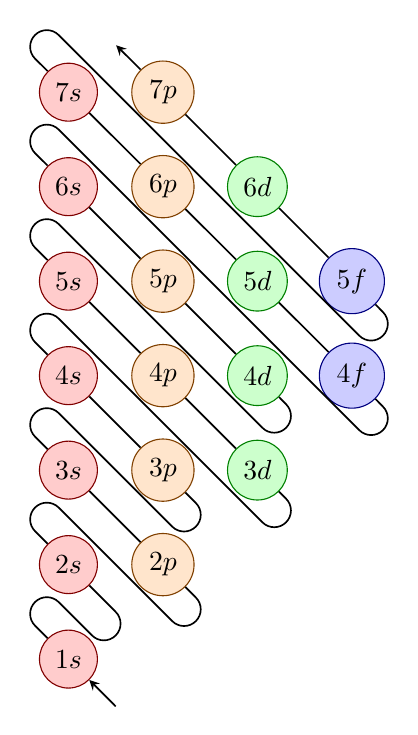
\begin{tikzpicture}[>=stealth,scale=1.2]
  \foreach \y in {1,...,7}
  {
    \node (s\y) at (0,\y) [circle,draw=red!50!black,fill=red!20]{$\y s$}; 
  }
  \foreach \y in {2,...,7}
  {
    \node (p\y) at (1,\y) [circle,draw=orange!50!black,fill=orange!20]{$\y p$};
  }
  \foreach \y in {3,...,6}
  {
    \node (d\y) at (2,\y) [circle,draw=green!50!black,fill=green!20]{$\y d$};
  }
  \foreach \y in {4,5}
  {
    \node (f\y) at (3,\y) [circle,draw=blue!50!black,fill=blue!20]{$\y f$};
  }
  \draw[semithick,->](s1)--++(135:0.5)arc(225:45:{sqrt(2)/8})--++(-45:0.5)arc(-135:45:{sqrt(2)/8})--(s2)
  --++(135:0.5)arc(225:45:{sqrt(2)/8})--++(-45:1.7)arc(-135:45:{sqrt(2)/8})--(p2)--(s3)
  --++(135:0.5)arc(225:45:{sqrt(2)/8})--++(-45:1.7)arc(-135:45:{sqrt(2)/8})--(p3)--(s4)
  --++(135:0.5)arc(225:45:{sqrt(2)/8})--++(-45:3.05)arc(-135:45:{sqrt(2)/8})--(d3)--(p4)--(s5)
  --++(135:0.5)arc(225:45:{sqrt(2)/8})--++(-45:3.05)arc(-135:45:{sqrt(2)/8})--(d4)--(p5)--(s6)
  --++(135:0.5)arc(225:45:{sqrt(2)/8})--++(-45:4.5)arc(-135:45:{sqrt(2)/8})--(f4)--(d5)--(p6)--(s7)
  --++(135:0.5)arc(225:45:{sqrt(2)/8})--++(-45:4.5)arc(-135:45:{sqrt(2)/8})--(f5)--(d6)--(p7)--++(135:0.7);
  \draw[semithick,->](0.5,0.5)--(s1);
\end{tikzpicture}
\end{document}